\section{The Agentic Framework}

In this section, we provide a conceptual overview of the framework we develop,
and describe its implementation in Python.

\subsection{Conceptual Model}

The goal of our framework is to enable the development of the \emph{agentic
flows} as described in the AgentInstruct \citep{mitra_agentinstruct_2024} paper.
At a high level, an agentic flow describes the transformation of initial seed
data into fine-tune examples by computations of coordinating agents.

We initially considered basing our conceptual model on prior work on agentic
frameworks, such as AutoGen \cite{wu2023autogenenablingnextgenllm} and
LangChain's LangGraph \cite{langchain}. In such frameworks, agents are
event-based actors that, when they receive a message, perform some computations
and potentially communicate with other actors.

However, we found that for the purpose of developing agentic flows, this
conceptual model is overly general. In particular, the general agent model
treats the messages sent between agents as being first-class, the notion of data
being transformed is not captured by the model.

Therefore, we develop a new conceptual model that treats the stream of data
being transformed as first-class. Agents are (potentially nondeterministic)
\emph{functions} that manipulate the stream of data, and coordination between
agents occurs via an explicit graph topology. This model is inherently more
restrictive than the general conceptual model, however, there restrictions
enable greater composability. In particular agents for common stream operations
(e.g. \texttt{map} or \texttt{filter}) can easily be composed to form complex
pipelines. In our Python implementation, we provide implementations of such
general-purpose agents.

\subsubsection{Core Concepts}

Our resulting framework is based around three key concepts: \emph{streams},
\emph{agents}, and \emph{pipelines}. A \emph{stream} $\stream{\mathcal{T}}$ is a
potentially infinite list of values of some type $\mathcal{T}$; for example, the
list of numbers in the range $[0, 10]$ is a stream $\stream{\mathbb{N}}$.

An \emph{agent} $\agent : \streamty{\mathcal{T}} \rightarrow
\streamty{\mathcal{U}}$ is a nondeterministic function that maps an \emph{input
stream} $\stream{\mathcal{T}}$ to an output stream $\stream{\mathcal{U}}$, we
use $\agentin{\agent}$ and $\agentout{\agent}$ to denote the type of $\agent$'s
input and output streams respectively.

A \emph{pipeline} is a connected directed graph of agents, containing a
unique \emph{source agent} $\agent{}_{\mathit{source}}$ and a unique \emph{sink
agent} $\agent_{\mathit{sink}}$. We note that the source and sink agent are not
necessarily distinct: the simplest pipeline is one consisting of a single agent.
A pipeline defines a nondeterminstic function that maps a stream of type
$\agentin{\agent_{\mathit{source}}}$ to a stream of type
$\agentin{\agent_{\mathit{sink}}}$.

\subsection{Python Implementation}

We implement our framework in Python. In the design of our implementation, we
sought to achieve the following goals:

\begin{enumerate}
  \item The framework should enable a small semantic gap \cite{semanticgap}
  between user's intentions and the representation in code
  \item It should enable the development of efficient data pipelines that include
  e.g. parallelism and caching
\end{enumerate}

As in our conceptual model, streams are a key concept in our library: a stream
$\stream{T}$ is represented by an object of type \texttt{AsyncIterator[T]}. This
was a natural choice for our use case because \texttt{AsyncIterator} objects can
easily be created from data structures (esp. lists) and also directly defined
using Python's async generator syntax\footnote{For more details see
\url{https://peps.python.org/pep-0525/}}.

 The abstract class
\texttt{Pipeline[T, U]} implements pipelines, and declares the abstract method
\texttt{process : AsyncIterator[T] -> AsyncIterator[U]}. Agents are realized in
our implementation by the abstract class \texttt{Agent[T, U]} (which extends the
\texttt{Pipeline[T, U]} class).

Our library includes built-in TODO continue this part

\begin{itemize}
  \item Quick summary of the methodology
\end{itemize}

In this section, we introduce our framework for generating synthetic data and fine-tuning LLMs on that data.
We also discuss the evaluation approach used to compare the performance of LLMs fine-tuned via our framework
with traditional RAG-based techniques.


\subsection{Framework Architecture}
\begin{itemize}
  \item Talk about the prompts and algorithm used to generate synthetic data
\end{itemize}

Our initial research drew inspiration from agentic-based frameworks like AgentInstruct % \citep{mitra_agentinstruct_2024};
however during the development of our framework, we found opportunities to leverage a more streamlined and efficient approach.
We developed a pipeline architecture that introduces more precise controls over the
synthetic data generation process while leveraging the power of small language models to create accurate
and diverse synthetic data based on seed data.

The pipeline consists of three main components: the \textit{Question Generator}, the \textit{Answer Generator}, and the \textit{QA Refinement Generator}.

\begin{figure}[h]
  \centering
  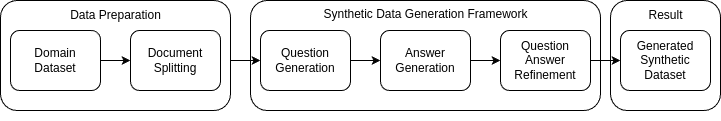
\includegraphics[width=\textwidth]{methodology-overview.png}
  \caption{An overview of our synthetic data generation framework. Given a user-provided domain dataset, our
framework will employ small language models to create a synthetic dataset that can be used
to fine-tune a SLM for downstream Question Answering tasks.}
\end{figure}

\subsubsection{Data Preparation}
For the source dataset used in our framework, we used ArXiv papers published after 2024, specifically papers relevant to
small language models, fine-tuning LLM's and synthetic data generation.
This choice was motivated by several factors including:
\begin{itemize}
  \item Recent papers ensure that the content was not part of the pre-training data for the LLMs used in our framework
  \item The ease of access to the dataset, which is publicly available and well-structured
  \item Academic papers provide structured factual content that can be used to generate questions and answers and as a proxy for
  domain-specific data in other applications
\end{itemize}

To prepare the data into our framework, we chunked each paper into a fixed size and extracted the title to be used in the
question generator.

\subsubsection{Question Generator}

In the first step of the pipeline, the Question Generator takes the title of the paper along with a chunk of text from the paper
and generates an initial set of questions that can be answered using the text. To facilitate the generation of diverse questions,
we used a small language model to generate a mix of 'what', 'why', 'how', 'where', and 'summarize' questions, the full prompt can be found in the appendix?.

For each question in our framework, we ensure that the title information is included in the question to serve as context during fine-tuning. We hypothesize
that by including the title in the question, the model will be able to better retrieve the correct answer during downstream zero-shot question answering tasks on the fine-tuned
model. Intuitively, this serves as a form of conditioning for the language model during generation. <Should prove this with some data or results>

To minimize generating duplicate or similar questions, we leverage a similarity check using the cosine similarity between the embeddings of the generated questions
and remove questions that have high similar.

\subsubsection{Answer Generator}

Following the generation of questions, the Answer Generator takes the generated questions and the corresponding text chunk and generates answers for each of the questions.
In this step, we prioritize factual accuracy, organized structure of the response, and clarity. This step can be seen as a simple form of question answering, where the model is
tasked with generating the answer to a question given the context of the text chunk.

\subsubsection{QA Refinement Generator}

To refine each question-answer pair, we generate a new set of questions that are based on the original question and the answer pair
with the goal of generating questions that approaches the original question from a different angle. This step is critical in
generating more qa pairs while also generating questions that are more challenging and involve more reasoning than the original question.

We generate an answer for each of the refined questions using a similar process as the Answer Generator but using the original answer
and smaller chunks retrieved from a similarity search as context. The extra step in retrieving smaller chunks of text is to ensure that the model
has context to answer the question that is not directly in the original text chunk. Intuitively, we take inspiration from Retrieval Augmented Generation
(RAG) frameworks using vector databases to generate answers in the QA Refinement Generator.

\subsubsection{Result}

Upon completion of the pipeline, we have a set of question-answer pairs that can be used to fine-tune a small language model for downstream QA tasks.
We perform simple heuristics to ensure that questions that could not be answered or may not exist in the original text are removed from the dataset.

\subsection{Algorithm}
\begin{itemize}
  \item Maybe breaking this out into an algorithm or a flowchart
\end{itemize}

